% Options for packages loaded elsewhere
\PassOptionsToPackage{unicode}{hyperref}
\PassOptionsToPackage{hyphens}{url}
%
\documentclass[
]{article}
\usepackage{amsmath,amssymb}
\usepackage{lmodern}
\usepackage{ifxetex,ifluatex}
\ifnum 0\ifxetex 1\fi\ifluatex 1\fi=0 % if pdftex
  \usepackage[T1]{fontenc}
  \usepackage[utf8]{inputenc}
  \usepackage{textcomp} % provide euro and other symbols
\else % if luatex or xetex
  \usepackage{unicode-math}
  \defaultfontfeatures{Scale=MatchLowercase}
  \defaultfontfeatures[\rmfamily]{Ligatures=TeX,Scale=1}
\fi
% Use upquote if available, for straight quotes in verbatim environments
\IfFileExists{upquote.sty}{\usepackage{upquote}}{}
\IfFileExists{microtype.sty}{% use microtype if available
  \usepackage[]{microtype}
  \UseMicrotypeSet[protrusion]{basicmath} % disable protrusion for tt fonts
}{}
\makeatletter
\@ifundefined{KOMAClassName}{% if non-KOMA class
  \IfFileExists{parskip.sty}{%
    \usepackage{parskip}
  }{% else
    \setlength{\parindent}{0pt}
    \setlength{\parskip}{6pt plus 2pt minus 1pt}}
}{% if KOMA class
  \KOMAoptions{parskip=half}}
\makeatother
\usepackage{xcolor}
\IfFileExists{xurl.sty}{\usepackage{xurl}}{} % add URL line breaks if available
\IfFileExists{bookmark.sty}{\usepackage{bookmark}}{\usepackage{hyperref}}
\hypersetup{
  pdftitle={Group\_01\_Project2\_demo},
  pdfauthor={Group\_01},
  hidelinks,
  pdfcreator={LaTeX via pandoc}}
\urlstyle{same} % disable monospaced font for URLs
\usepackage[margin=1in]{geometry}
\usepackage{graphicx}
\makeatletter
\def\maxwidth{\ifdim\Gin@nat@width>\linewidth\linewidth\else\Gin@nat@width\fi}
\def\maxheight{\ifdim\Gin@nat@height>\textheight\textheight\else\Gin@nat@height\fi}
\makeatother
% Scale images if necessary, so that they will not overflow the page
% margins by default, and it is still possible to overwrite the defaults
% using explicit options in \includegraphics[width, height, ...]{}
\setkeys{Gin}{width=\maxwidth,height=\maxheight,keepaspectratio}
% Set default figure placement to htbp
\makeatletter
\def\fps@figure{htbp}
\makeatother
\setlength{\emergencystretch}{3em} % prevent overfull lines
\providecommand{\tightlist}{%
  \setlength{\itemsep}{0pt}\setlength{\parskip}{0pt}}
\setcounter{secnumdepth}{-\maxdimen} % remove section numbering
\usepackage{booktabs}
\usepackage{longtable}
\usepackage{array}
\usepackage{multirow}
\usepackage{wrapfig}
\usepackage{float}
\usepackage{colortbl}
\usepackage{pdflscape}
\usepackage{tabu}
\usepackage{threeparttable}
\usepackage{threeparttablex}
\usepackage[normalem]{ulem}
\usepackage{makecell}
\usepackage{xcolor}
\ifluatex
  \usepackage{selnolig}  % disable illegal ligatures
\fi

\title{Group\_01\_Project2\_demo}
\author{Group\_01}
\date{}

\begin{document}
\maketitle

\hypertarget{sec:Intro}{%
\section{Introduction}\label{sec:Intro}}

Data come from the FIES (Family Income and Expenditure Survey) recorded
in the Philippines. The survey, which is undertaken every three years,
is aimed at providing data on family income and expenditure. The data
obtained from this survey are from different regions across the
Philippines.

In particular, this report further explores how does total household
income, total foods expenditure, household head's sex, household head's
age, type of household, house floor area, house age, number of bedrooms
and electricity infect the number of family members.

\hypertarget{sec:EDA}{%
\section{Exploratory Data Analysis}\label{sec:EDA}}

Table 1 shows summary data for all the variables from the FIES (Family
Income and Expenditure Survey) data. First, the total number of family
members ranges from 1 to 15, with the middle 50\% of number of family
members falling between 3 and 6 also an average number of family members
of 4.67. Secondly, the total household income is range from 11988 to
6042860. The middle 50\% of total household income is between 118565 and
328335, with 269540.48 on average. Next, we may look at the total food
expenditure, which is the range of 6781 to 327724, with the middle 50\%
lies between 51922 and 98493. Then,

\begin{table}

\caption{\label{tab:numerical summaries}Summary statistics of numerical variables}
\centering
\resizebox{\linewidth}{!}{
\fontsize{10}{12}\selectfont
\begin{tabular}[t]{lrrrrrrrrr}
\toprule
Variable & Missing & Complete & Mean & SD & Min. & 1st Q. & Median & 3rd Q. & Max.\\
\midrule
Total.Number.of.Family.members & 0 & 1 & 4.67 & 2.33 & 1 & 3 & 4 & 6 & 15\\
Total.Household.Income & 0 & 1 & 269540.48 & 274564.17 & 11988 & 118565 & 188580 & 328335 & 6042860\\
Total.Food.Expenditure & 0 & 1 & 80352.78 & 41194.36 & 6781 & 51922 & 73578 & 98493 & 327724\\
Household.Head.Age & 0 & 1 & 52.23 & 14.52 & 17 & 41 & 52 & 63 & 99\\
House.Floor.Area & 0 & 1 & 90.92 & 99.20 & 5 & 32 & 54 & 102 & 900\\
\addlinespace
House.Age & 0 & 1 & 22.98 & 15.32 & 0 & 12 & 20 & 31 & 100\\
Number.of.bedrooms & 0 & 1 & 2.26 & 1.44 & 0 & 1 & 2 & 3 & 9\\
Electricity & 0 & 1 & 0.93 & 0.26 & 0 & 1 & 1 & 1 & 1\\
\bottomrule
\end{tabular}}
\end{table}

Figure 1 shows the distribution of the total number of family members.
This distribution plot shows that the number of family members fitts
poisson distribution.

\begin{center}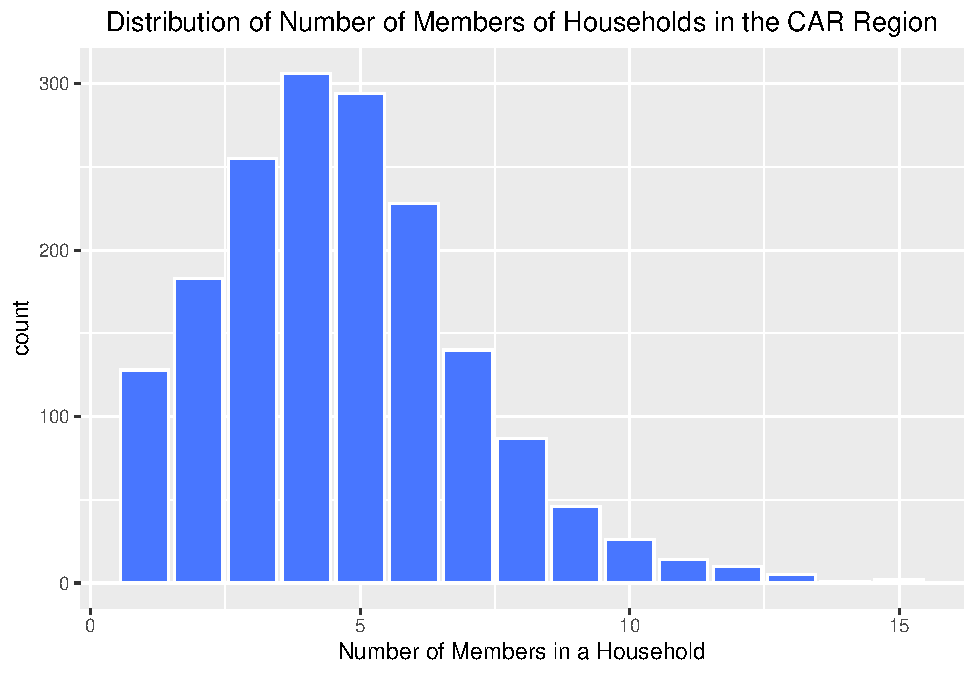
\includegraphics[width=0.8\linewidth]{Group_01_Project2_demo_files/figure-latex/distribution of response variable-1} \end{center}

The correlation coefficient between all variables shows in Table 2. The
correlation coefficient between total food expenditure and total number
of family members is 0.469, and the correlation coefficient between
total household income and total number of family members is 0.192. By
the way, the correlation coefficient between household Head's age, house
floor area, house age and total number of family members are negative,
which shows the rise of those three variables will lead to the decrease
of the total number of family members.

\begin{table}

\caption{\label{tab:correlation}Table 2: Correlation of all variables.}
\centering
\resizebox{\linewidth}{!}{
\fontsize{10}{12}\selectfont
\begin{tabular}[t]{lrrrrrrrr}
\toprule
  & Total.Number.of.Family.members & Total.Household.Income & Total.Food.Expenditure & Household.Head.Age & House.Floor.Area & House.Age & Number.of.bedrooms & Electricity\\
\midrule
Total.Number.of.Family.members & 1.000 & 0.192 & 0.469 & -0.065 & -0.014 & -0.070 & 0.072 & 0.092\\
Total.Household.Income & 0.192 & 1.000 & 0.611 & 0.063 & 0.234 & 0.025 & 0.441 & 0.149\\
Total.Food.Expenditure & 0.469 & 0.611 & 1.000 & -0.052 & 0.124 & 0.007 & 0.356 & 0.199\\
Household.Head.Age & -0.065 & 0.063 & -0.052 & 1.000 & 0.091 & 0.218 & 0.154 & -0.013\\
House.Floor.Area & -0.014 & 0.234 & 0.124 & 0.091 & 1.000 & 0.074 & 0.374 & 0.107\\
\addlinespace
House.Age & -0.070 & 0.025 & 0.007 & 0.218 & 0.074 & 1.000 & 0.123 & 0.085\\
Number.of.bedrooms & 0.072 & 0.441 & 0.356 & 0.154 & 0.374 & 0.123 & 1.000 & 0.214\\
Electricity & 0.092 & 0.149 & 0.199 & -0.013 & 0.107 & 0.085 & 0.214 & 1.000\\
\bottomrule
\end{tabular}}
\end{table}

\begin{figure}

{\centering 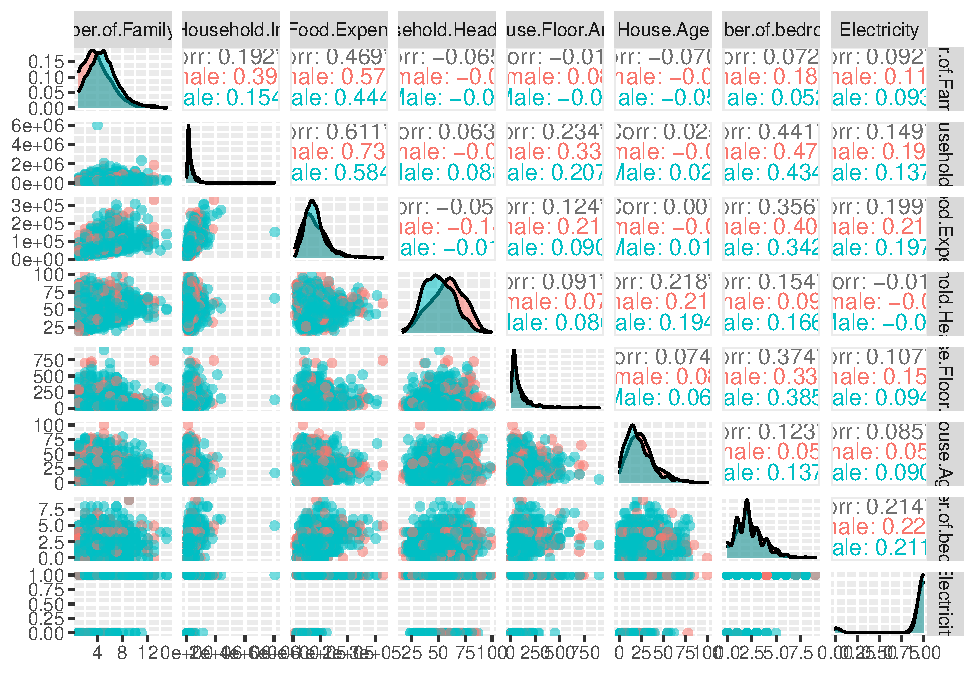
\includegraphics[width=1\linewidth]{Group_01_Project2_demo_files/figure-latex/pairs-1} 

}

\caption{Figrue 3: Paired plots of the variables}\label{fig:pairs}
\end{figure}

\end{document}
